% Small schematic of the x85 crossed design: 96 prompts x 24 harm/neutral
% word pairs, one cell = prompt with one word appended; the neutral-corrected
% boundary difference D[p,w] = h(H) - h(N); the shared direction is fitted
% with prompt AND word folds held out and evaluated on the unseen quadrant.
% Facts from knowledge/experiments/x85-crossed-keyword-prompt-latent-decomposition.md.
%
% Compile (from the repository root; the paper includes it as crossed-grid.pdf):
%   pdflatex -output-directory=figures -jobname=crossed-grid code/figures/fig-crossed.tex
\documentclass[tikz,border=2pt]{standalone}
\usepackage[T1]{fontenc}
\usepackage{amsmath}
\usetikzlibrary{positioning,arrows.meta,calc}

\definecolor{cblue}{HTML}{0072B2}
\definecolor{corange}{HTML}{E69F00}
\definecolor{ink}{HTML}{333333}
\definecolor{muted}{HTML}{888888}
\definecolor{paleblue}{HTML}{EAF3F9}
\definecolor{palegray}{HTML}{F0F0F0}

\newcommand{\csz}{0.52}% cell size, cm

\begin{document}
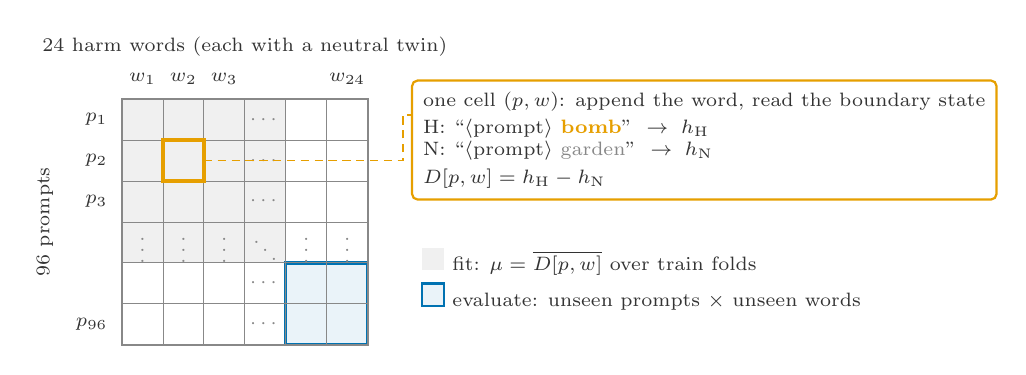
\begin{tikzpicture}[
  font=\scriptsize\color{ink},
  flow/.style={-{Stealth[length=2mm]}, thick, draw=ink},
  lab/.style={font=\scriptsize\color{ink}},
  mut/.style={font=\scriptsize\color{muted}},
]

% ---- Grid: rows = prompts, columns = word pairs -----------------------------
% 6x6 displayed cells; row/col 4 are ellipses; last two rows/cols = held-out.
\begin{scope}
  % fit region (all cells except held-out rows/cols)
  \fill[palegray] (0,0) rectangle (4*\csz, -4*\csz);
  % evaluation quadrant: unseen prompt x unseen word
  \fill[paleblue] (4*\csz,-4*\csz) rectangle (6*\csz,-6*\csz);
  \draw[cblue, very thick] (4*\csz,-4*\csz) rectangle (6*\csz,-6*\csz);
  % grid lines
  \draw[muted, line width=0.3pt] (0,0) grid[step=\csz cm] (6*\csz,-6*\csz);
  \draw[muted, thick] (0,0) rectangle (6*\csz,-6*\csz);

  % ellipses inside cells (4th row/col)
  \foreach \r in {1,2,3,5,6} {
    \node[mut] at (3.5*\csz, {-(\r-0.5)*\csz}) {$\cdots$};
    \node[mut] at ({(\r-0.5)*\csz}, -3.5*\csz) {$\vdots$};
  }
  \node[mut] at (3.5*\csz,-3.5*\csz) {$\ddots$};

  % column labels: word pairs
  \node[lab, anchor=south] at (0.5*\csz, 0.06) {$w_1$};
  \node[lab, anchor=south] at (1.5*\csz, 0.06) {$w_2$};
  \node[lab, anchor=south] at (2.5*\csz, 0.06) {$w_3$};
  \node[lab, anchor=south] at (5.5*\csz, 0.06) {$w_{24}$};
  % row labels: prompts
  \node[lab, anchor=east] at (-0.06, -0.5*\csz) {$p_1$};
  \node[lab, anchor=east] at (-0.06, -1.5*\csz) {$p_2$};
  \node[lab, anchor=east] at (-0.06, -2.5*\csz) {$p_3$};
  \node[lab, anchor=east] at (-0.06, -5.5*\csz) {$p_{96}$};

  % axis titles
  \node[lab, anchor=south] at (3*\csz, 0.42)
    {24 harm words (each with a neutral twin)};
  \node[lab, anchor=south, rotate=90] at (-0.75, -3*\csz) {96 prompts};
\end{scope}

% one highlighted train cell for the zoom
\draw[corange, very thick] (1*\csz,-1*\csz) rectangle (2*\csz,-2*\csz);
\draw[corange, densely dashed, line width=0.5pt] (2*\csz,-1.5*\csz) -- (6*\csz+0.45, -1.5*\csz)
  -- (6*\csz+0.45, -0.2) -- (6*\csz+0.55, -0.2);

% ---- Zoom: what one cell is -------------------------------------------------
\node[draw=corange, thick, rounded corners=2pt, fill=white, align=left,
      anchor=north west, inner sep=4pt] (zoom) at (6*\csz+0.55, 0.25) {%
  one cell $(p, w)$: append the word, read the boundary state\\[2pt]
  H:\ ``$\langle$prompt$\rangle$ {\bfseries\color{corange}bomb}''
      $\;\rightarrow\; h_{\mathrm{H}}$\\
  N:\ ``$\langle$prompt$\rangle$ {\color{muted}garden}''
      $\;\rightarrow\; h_{\mathrm{N}}$\\[2pt]
  $D[p,w] = h_{\mathrm{H}} - h_{\mathrm{N}}$};

% ---- Legend / readout -------------------------------------------------------
\node[align=left, anchor=north west] (legend) at (6*\csz+0.55, -6*\csz+1.35) {%
  \begin{tabular}{@{}c@{\ }l@{}}
  \tikz\fill[palegray] (0,0) rectangle (0.28,0.28); &
    fit: $\mu = \overline{D[p,w]}$ over train folds\\[2pt]
  \tikz{\fill[paleblue] (0,0) rectangle (0.28,0.28);
        \draw[cblue, thick] (0,0) rectangle (0.28,0.28);} &
    evaluate: unseen prompts $\times$ unseen words\\
  \end{tabular}};

\end{tikzpicture}
\end{document}
